\section{Variational Autoencoder}
Variational Autoencoders, basing on the architecture of neural networks heavily, will have a lot in common in terms of the way they work. This section will focus on the aspects that are unique to VAE, and if possible — compare with AE. Again, useful assumptions were made:
\begin{itemize}
    \item the architecture used for both encoder and decoder is a multilayer perceptron with 2 layers and a hidden size of $128$, and the latent size (between the encoder and the decoder) of $10$,
    \item learning was conducted for $20$ epochs, with batch size $64$ and Adam optimizer with learning rate of $1*10^{-3}$, 
    \item a subset of $10000$ samples from the $28\textrm{x}28$ MNIST dataset was used.
\end{itemize}

\subsection{Latent separability}
Latent separability in autoencoders shows how much the representation is able to distinguish between classes (please note that this is not identical to being disentangled, which needs a different type of measurement \cite{Higgins2017}). In \autoref{fig:vae-separability} a \textit{t-distributed stochastic neighbor embedding} (t-SNE) of autoencoder and variational autoencoder representations were shown. Labels of particular classes were saved and annotated on the plots for easier comparability. While the main goal of t-SNE is to capture structure (in the sense that neighboring points in the input space will tend to be neighbors in the low dimensional space). While not deterministic, it preserves the clusters together (although it does not preserve distances) \cite{Hinton2009}.

\vspace{\baselineskip}
That being said, it can be seen that both AE and VAE do cope with latent separability similarly. Classes that are separated the best are $0$, $1$, $6$. They also have issues with the same two groups of classes, and there is not much difference in intensity of the error.

\begin{figure}[]
     \centering
     \begin{subfigure}[b]{0.48\textwidth}
         \centering
         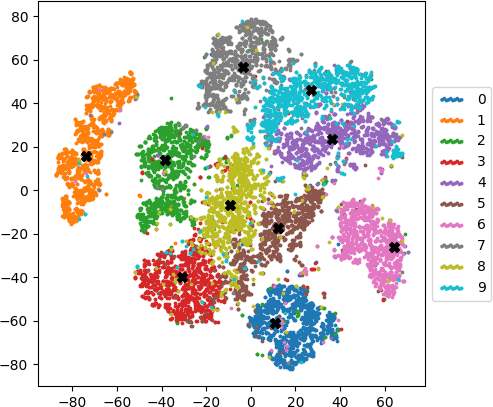
\includegraphics[width=\textwidth]{observational/img/vae/ae_tsne.png}
         \caption{t-SNE of the AE representation}
     \end{subfigure} 
     \hfill
     \begin{subfigure}[b]{0.48\textwidth}
          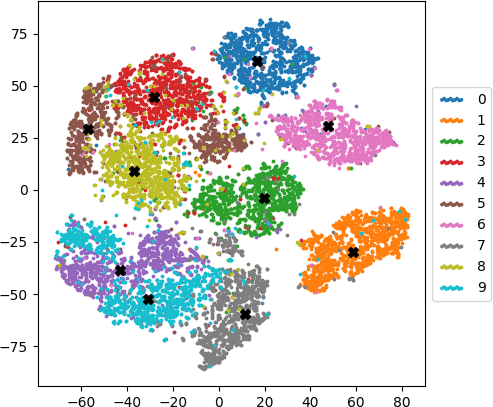
\includegraphics[width=\textwidth]{observational/img/vae/vae_tsne.png}
         \caption{t-SNE of the VAE representation}
     \end{subfigure} 
     \caption[Comparison of AE and VAE latent separation]{A comparison of Autoencoder (a) and Variational Autoencoder (b) t-SNE separation of representation.}
    \label{fig:vae-separability}
\end{figure}

\subsection{Latent space quality}
One of the most significant features of the well-trained autoencoders is being able to reconstruct the input from the latent space. Similarly to conventional neural networks, classical autoencoders cannot represent many latent vectors, as only one must be selected. Variational autoencoders, on the other hand, learn a distribution, thus (at least in theory) retain more information, which should result in better quality latent space, and thus input reconstruction.

\vspace{\baselineskip}
This hypothesis proves true in latent space visualizations in \autoref{fig:vae-latent-viz}. They were prepared by reconstructing (passing through the decoder) the latent space. Presented images are a result of visualizing features for a latent code of digit $9$. It is visible that particular squares are of higher quality in the VAE's space. The digits are more robust, well-defined and less blurry. Additionally, more of them resemble the actual digit $9$.

\begin{figure}[]
     \centering
     \begin{subfigure}[b]{0.49\textwidth}
         \centering
         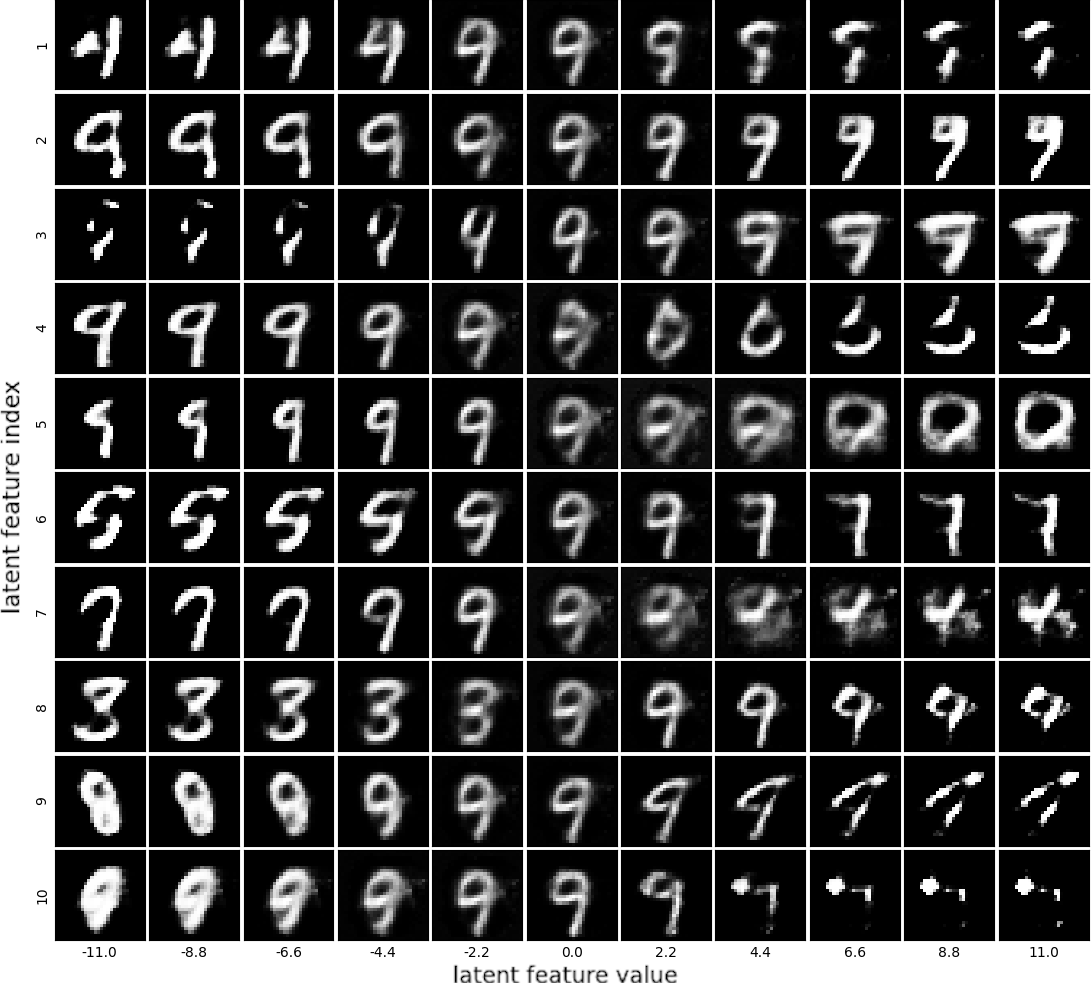
\includegraphics[width=\textwidth]{observational/img/vae/ae_latent_viz.png}
         \caption{AE — latent visualization}
     \end{subfigure} 
     \hfill
     \begin{subfigure}[b]{0.49\textwidth}
          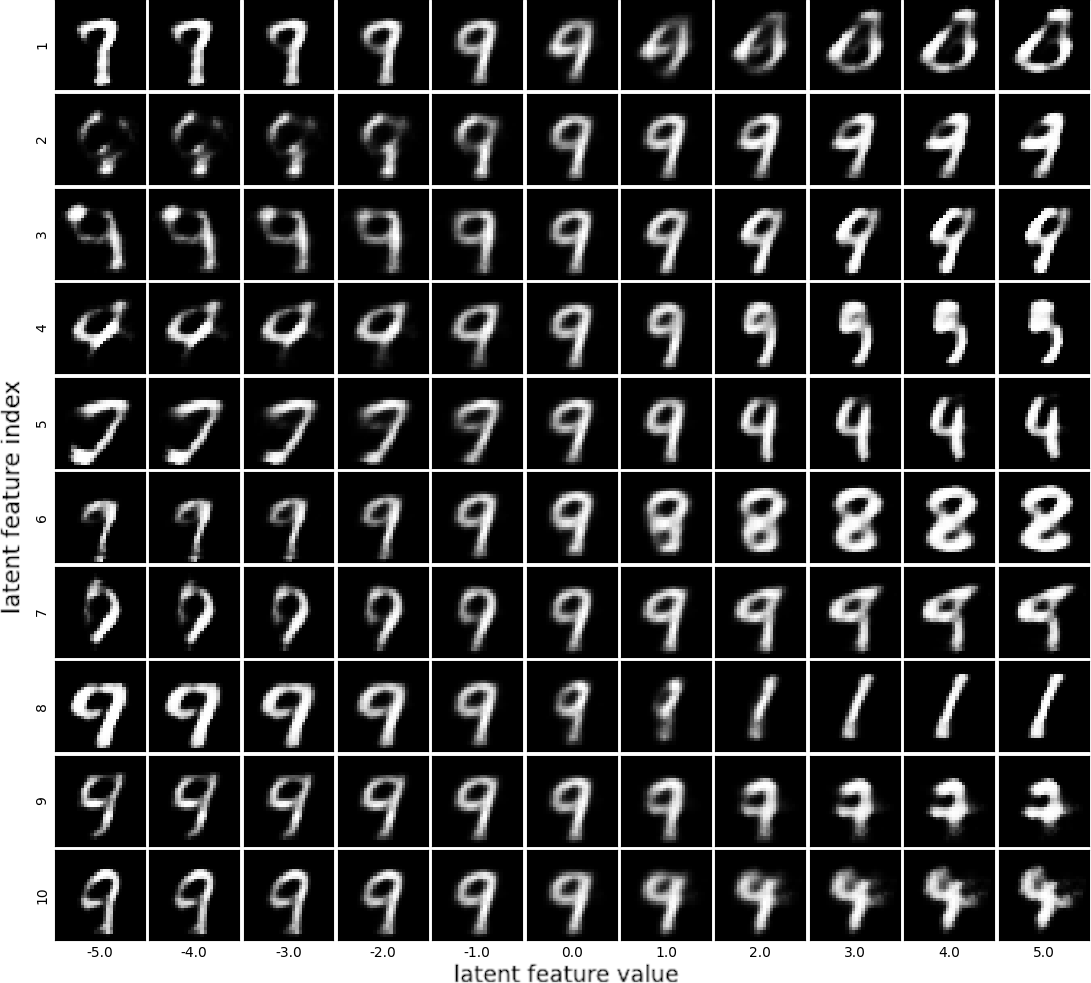
\includegraphics[width=\textwidth]{observational/img/vae/vae_latent_viz.png}
         \caption{VAE — latent visualization}
     \end{subfigure} 
     \caption[Comparison of AE and VAE latent visualizations]{A comparison of Autoencoder (a) and Variational Autoencoder (b) latent space visualizations. Presented images are a result of visualizing features for a latent code of digit $9$.}
    \label{fig:vae-latent-viz}
\end{figure}

\vspace{\baselineskip}
A similar observation can be made in \autoref{fig:vae-avg-reconstruction}, where average reconstructions of the input were presented. 

\begin{figure}[]
     \centering
     \begin{subfigure}[b]{0.45\textwidth}
         \centering
         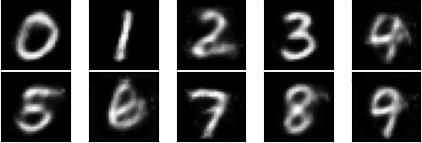
\includegraphics[width=\textwidth]{observational/img/vae/ae_avg_reconstruction.png}
         \caption{AE — average input reconstruction}
     \end{subfigure} 
     \hfill
     \begin{subfigure}[b]{0.45\textwidth}
          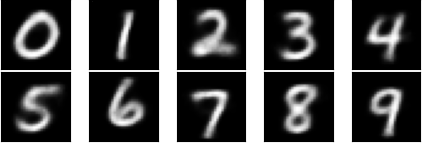
\includegraphics[width=\textwidth]{observational/img/vae/vae_avg_reconstruction.png}
         \caption{VAE — average input reconstruction}
     \end{subfigure} 
     \caption[Comparison of AE and VAE average input reconstructions]{A comparison of Autoencoder (a) and Variational Autoencoder (b) average input reconstructions.}
    \label{fig:vae-avg-reconstruction}
\end{figure}


\subsection{Latent size analysis}
A discussion on the importance of latent representations cannot neglect an inherent aspect of it — the size and how it influences its quality. For that reason, two experiments have been conducted. Both separability and quality of the latent space was compared over different latent sizes.

\vspace{\baselineskip}
\autoref{fig:vae-tsne-latent} shows t-SNE visualizations over a range of latent sizes. Too large values cause the clusters to scatter and fuse, which is a sign of poor separability — the larger the value, the bigger spread occurs. Excessively small values will obtain highly separated clusters. While the elongated curve-like shape of clusters for the size equal to $1$ is not necessarily an issue (it is simply a result of how t-SNE processes data), the heavy mixing of classes within those clusters can raise some doubts.

\vspace{\baselineskip}
To supplement the separability analysis, \autoref{fig:vae-latent-recon} provides averages of input reconstructions for each class. In general, larger values yield better results (though a slight regression is visible for excessively large ones). With the increase of the latent size, the numbers seem less blurry and more recognizable (with the lowest values being almost illegible). Due to the trend being reverse to that from the separability analysis, the middle values seem optimal and because they are not fixed, the latent size should be treated as a hyperparameter.

\include*{observational/vae_tsne}
\include*{observational/vae_avg_reconstruction}